\documentclass[a4paper,12pt]{article}

\usepackage{graphicx}   % For including images
\usepackage{setspace}   % For line spacing
\usepackage{geometry}   % To adjust margins
\usepackage{ragged2e}
\usepackage{array}
\usepackage{caption}
\geometry{margin=1in}   % Set margin size
\usepackage{subcaption}

\begin{document}

\begin{center}
    \textbf{\huge{CS702 - COMPUTING LAB}} \vspace{2cm}

    \Large{A REPORT ON THE PROJECT ENTITLED} \vspace{1cm}

    \textbf{\LARGE{COVERSATIONAL USED CAR PRICE PREDICTOR}} \vspace{2cm}
\end{center}

\begin{center}
    \includegraphics[width=0.3\textwidth]{logo.jpeg} % Specify the path to your logo image
\end{center}

\vfill

\noindent
\begin{center}
    \textbf{Group Members:} \\
    \vspace{0.5cm}  % Adds a bit of vertical space
    \begin{tabular}{c @{\hspace{3cm}} c}  % Creates two columns with 3cm space between them
        \textbf{ABHIJITH C} & \textbf{ANAND M K} \\
        \textbf{242CS003} & \textbf{242CS008} \\
    \end{tabular}
\end{center}

\vfill

\begin{center}
    \textbf{I SEMESTER M-TECH CSE} \vspace{2cm}

    \textbf{DEPARTMENT OF COMPUTER SCIENCE AND ENGINEERING}
	
    \textbf{NATIONAL INSTITUTE OF TECHNOLOGY KARNATAKA}

    \textbf{SURATHKAL}

    \textbf{2024 – 2025}
\end{center}

\newpage
\tableofcontents
\newpage

\section{Introduction}
\begin{justify}
Conversational interfaces are becoming increasingly important in making human interactions with technology more natural and easy to use. These systems use Natural Language Processing (NLP) technology to understand user inputs and respond appropriately.

With the rising demand for used cars, many consumers face challenges in accurately determining the value of a vehicle, often due to a lack of information or expertise. This is where Machine Learning-based price prediction plays a vital role.

The goal of this project is to create a conversational interface that gathers key details from users to predict the price of their used car. The prediction model will use this information to estimate the car’s price, which will then be communicated to the user through the interface.
\newline
\end{justify}


\section{Problem Statement and Objectives}
\begin{justify}
Accurately predicting the price of a used car involves gathering and analyzing a variety of details, such as the car's brand, model, year, mileage, and other factors. Traditional methods for this, like filling out forms, can feel tedious and impersonal, leading to a poor user experience.

This project aims to address these issues by developing a Conversational Used Car Price Predictor that integrates a chatbot interface with a machine learning model. The goal is to enable users to interact naturally through conversation, rather than filling out forms, to predict the price of a used car. The chatbot will guide users step-by-step to collect necessary car details and will handle additional queries, such as explaining how the predicted price was calculated or which factors most affect the car's value.

By making the process more intuitive and engaging, this system aims to improve user experience and deliver accurate and reliable price predictions.
\end{justify}

\section{Literature Survey}

\begin{table}[ht]
\centering
\footnotesize
\begin{tabular}{|c|m{6cm}|c|m{6cm}|}
    \hline
    \textbf{S.No.} & \textbf{Title} & \textbf{Year} & \textbf{Methodology} \\ \hline
    1 & Prediction of Used Car Prices Using Artificial Neural Networks and Machine Learning & 2022 & Deep Neural Networks, Linear Regression, Random Forest Algorithm \\ \hline
    2 & Predicting the Sale Price of Pre-Owned Vehicles with the Ensemble ML Model & 2023 & Linear Regression Model, Random Forest Regression, Gradient Boosting Tree (GBT) Regression Model \\ \hline
    3 & An Overview of Chatbot Technology & 2020 & Rule-Based Model Chatbots, Generative Models. Development platforms can be open-source, such as RASA. \\ \hline
    4 & Conversational AI Unleashed: A Comprehensive Review of NLP-Powered Chatbot Platforms & 2023 & Rule-Based Systems, Generative Models. \\ \hline
    5 & Framework for Design and Implementation of Chat Support System using Natural Language Processing & 2023 & The chatbot is developed in Django web framework and spaCy NLP library for Python. \\ \hline
\end{tabular}
\label{table:lit_survey}
\caption{\footnotesize Summary of Related Work in Used Car Price Prediction and Chatbot Development}
\end{table}


\section{System Architecture}
The system architecture for the \textit{Conversational Used Car Price Predictor} is designed to provide an interactive, user-friendly interface for estimating used car prices. The key components of the system include the \textit{Conversational Interface (Frontend)}, \textit{Rasa Engine}, \textit{Backend}, and the \textit{Price Prediction Model}, as shown in Figure~\ref{fig:architecture}.

\begin{figure}[h]
    \centering
    \includegraphics[width=0.8\textwidth]{Midsem.drawio.png}
    \caption{System Architecture of the Conversational Used Car Price Predictor}
    \label{fig:architecture}
\end{figure}

The system works as follows:
\begin{enumerate}
    \item The user interacts with the system via a conversational interface in the frontend, providing details such as the car’s make, model, year, mileage, and other relevant information.
    \item These inputs are processed by the \textbf{Rasa Engine}, which handles Natural Language Processing (NLP) and conversation management.
    \item The \textbf{Rasa Engine} extracts relevant parameters from the user's input and sends them to the backend via API calls.
    \item The backend forwards these parameters to the \textbf{Price Prediction Model}, which estimates the car's price based on the input features using a trained machine learning model.
    \item SHAP (SHapley Additive exPlanations) is applied to provide an explanation of how each input feature, such as mileage or car age, contributes to the predicted price.
    \item The backend returns both the predicted price and the explanation of the most significant contributing factor to the frontend.
    \item The predicted price and the SHAP-based explanation are then displayed to the user through the chat interface.
\end{enumerate}


\section{Data Preprocessing}
\begin{justify}
	Data preprocessing is a critical step to ensure that the machine learning model is provided with clean and well-structured data. Below are the detailed steps undertaken for preprocessing the dataset used in this project:
	
	\begin{itemize}
		\item \textbf{Dataset Acquisition}: The dataset for this project was sourced from \textbf{Kaggle} in 2023, under the name \texttt{cardekho\_dataset}. It contains a wide variety of features related to used cars, including attributes such as the brand, model, year, mileage, and selling price, which are essential for predicting the value of used cars.
		
		\item \textbf{Dropping Unnecessary Columns}: Certain columns in the dataset were deemed irrelevant or redundant for our analysis and were dropped. For example:
		\begin{itemize}
			\item The column \texttt{"Unnamed: 0"} was an irrelevant index and was removed.
			\item The \texttt{"car\_name"} and \texttt{seller\_type} columns, though informative, were redundant and did not contribute significantly to the model's predictive power.
		\end{itemize}
		
		\item \textbf{Converting Vehicle Age to Year of Manufacture}: To standardize the data, the \texttt{vehicle\_age} column was converted to \texttt{year\_of\_manufacture} using the formula:
		\[
		\texttt{year\_of\_manufacture} = 2023 - \texttt{vehicle\_age}
		\]
		After the conversion, the original \texttt{vehicle\_age} column was dropped.
		
		\item \textbf{Filtering Popular Car Models}: The dataset was filtered to retain only those car models that had more than 300 entries. This filtering ensures that the machine learning model is trained on a sufficiently large number of samples for each car model. The filtering process involved:
		\begin{itemize}
			\item Calculating the frequency of each car model using \texttt{value\_counts()}.
			\item Retaining only models with more than 300 entries to ensure robust model training.
		\end{itemize}
		
		\item \textbf{Feature and Target Definition}: For the machine learning model:
		\begin{itemize}
			\item \texttt{X} (features): Defined by dropping the column \texttt{selling\_price}.
			\item \texttt{y} (target): Defined as the \texttt{selling\_price} of the car, which the model aims to predict.
		\end{itemize}
		
		\item \textbf{Handling Categorical Columns}: Several features in the dataset were categorical, such as:
		\begin{itemize}
			\item \texttt{fuel\_type}
			\item \texttt{transmission\_type}
			\item \texttt{brand}
			\item \texttt{model}
		\end{itemize}
		These categorical variables needed to be converted into numerical format using encoding techniques for compatibility with machine learning algorithms. The \texttt{OneHotEncoder} was applied to these features to convert them into binary (0/1) variables.
		
		\item \textbf{Data Splitting}: The dataset was split into training and test sets in an 80:20 ratio using the \texttt{train\_test\_split()} function from \texttt{scikit-learn}. This ensures that the model is trained on 80\% of the data while the remaining 20\% is used to evaluate the model's performance. A \texttt{random\_state=42} was set to ensure reproducibility of results.
		
		\item \textbf{Preprocessing Pipeline}: To streamline preprocessing, a pipeline was implemented using \texttt{ColumnTransformer} from \texttt{scikit-learn}. This pipeline applies \texttt{OneHotEncoder} to categorical columns while allowing other features to pass through unchanged:
		\begin{quote}
			\texttt{ColumnTransformer(transformers=[('cat', OneHotEncoder(handle\_unknown='ignore', sparse\_output=False), categorical\_cols)], remainder='passthrough')}
		\end{quote}
		This preprocessing pipeline ensures that the categorical variables are encoded appropriately, making the data suitable for training the machine learning model.
		
	\end{itemize}
	
\end{justify}

\section{Model Training Process}
\begin{justify}
	The model training process involves selecting an appropriate machine learning algorithm, setting up a pipeline for preprocessing and model training, tuning hyperparameters, and evaluating the model's performance through cross-validation. Below is a detailed explanation of each step involved in training the car price prediction model.
	
	\begin{itemize}
		\item \textbf{Model Selection}: For this project, a \textbf{Random Forest Regressor} was chosen as the machine learning model for car price prediction. Random Forest is a powerful and flexible algorithm that handles both linear and non-linear relationships effectively. It is an ensemble learning method that constructs multiple decision trees during training and outputs the average prediction of the individual trees. This makes it robust and less prone to overfitting. Additionally, Random Forest works well with high-dimensional data and provides feature importance, making it suitable for our use case of price prediction.
		
		\item \textbf{Pipeline Setup}: To ensure seamless and consistent data processing during both the training and testing phases, a \textbf{pipeline} was created using the \texttt{Pipeline} class from \texttt{scikit-learn}. The pipeline integrates the preprocessing steps (such as One-Hot Encoding for categorical features) and the Random Forest model into a single workflow. This approach guarantees that the same transformations applied to the training data are also applied to the test data, thereby avoiding data leakage.
		
		\item \textbf{Hyperparameter Tuning}: To further optimize the performance of the Random Forest model, \textbf{RandomizedSearchCV} was employed for hyperparameter tuning. This method randomly samples a specified number of hyperparameter combinations from a predefined grid, allowing for efficient exploration of the hyperparameter space. The parameter grid for the Random Forest model included the following hyperparameters:
		\begin{itemize}
			\item \texttt{n\_estimators}: Number of trees in the forest, tested with values of 100, 200, and 300.
			\item \texttt{max\_depth}: The maximum depth of each tree, with possible values of \texttt{None}, 10, 20, and 30.
			\item \texttt{min\_samples\_split}: Minimum number of samples required to split an internal node, tested with values of 2, 5, and 10.
			\item \texttt{min\_samples\_leaf}: Minimum number of samples required to be at a leaf node, with values of 1, 2, and 4.
		\end{itemize}
		The number of iterations for the random search was set to \texttt{n\_iter=10}, meaning 10 different combinations of hyperparameters were randomly selected and evaluated.
		
		\item \textbf{Cross-Validation}: To ensure robust evaluation of the model's performance, \textbf{5-fold cross-validation} was used during hyperparameter tuning. In cross-validation, the data is split into 5 subsets (folds), and the model is trained on 4 of these folds while the remaining fold is used as the validation set. This process is repeated 5 times, with each fold serving as the validation set once. The model's performance is then averaged over the 5 iterations to give a more reliable estimate of how it will perform on unseen data.
		
		\item \textbf{Model Training and Evaluation}: Once the optimal hyperparameters were selected using RandomizedSearchCV, the final model was trained on the full training dataset. The model was then evaluated on the test set using the \textbf{R² score}, which measures the proportion of variance in the target variable (car prices) that is explained by the model. The best Random Forest model achieved an \textbf{R² score of 0.925} on the test set, indicating strong predictive performance.
		
		\item \textbf{Saving the Model}: To ensure that the trained model can be used for future predictions, it was saved using the \texttt{joblib} library. Saving the model allows for easy reuse without the need to retrain it every time a new prediction is required.
		
	\end{itemize}
	
\end{justify}


\section{Identifying Influential Features}
\begin{justify}
	One of the most valuable aspects of the machine learning model developed for predicting used car prices is its ability to provide explanations for its predictions. This is achieved using \textbf{SHAP} (SHapley Additive exPlanations), a method that assigns contribution values to each feature for a specific prediction. SHAP values allow us to break down and understand the role of each feature in driving the predicted price, offering insights into the decision-making process of the model.
	
	\begin{itemize}
		\item \textbf{SHAP Value Calculation}:
		Once the model is trained, SHAP values are computed for each prediction. SHAP values quantify how much each feature contributes to pushing the predicted price higher or lower than the average model output. For example, if a feature such as mileage has a positive SHAP value, it indicates that it pushes the predicted price higher; conversely, a negative SHAP value suggests that the feature lowers the predicted price.
		
		To compute SHAP values for this project, an \texttt{Explainer} object was created using the trained \texttt{RandomForestRegressor} model. The input data, after being transformed by the preprocessing pipeline, is passed to the explainer, which returns the SHAP values for each feature. These values represent how much each feature contributed to the predicted price for that particular car.
		
		\item \textbf{Analyzing SHAP Values}:
		The SHAP values are organized into a \texttt{DataFrame} for easy interpretation. This provides a clear breakdown of each feature’s contribution to the predicted price. Features with positive SHAP values are identified as those that increase the predicted price, while those with negative SHAP values reduce the predicted price. The SHAP values are computed for each car, allowing for an in-depth analysis of individual predictions.
		
		For instance, consider a test car such as the \textbf{BMW X5} (2020, Diesel, Automatic). The SHAP values provide insight into how much features like mileage, engine capacity, and fuel type contribute to the predicted price. This breakdown is valuable because it allows users to understand the key factors driving the price estimate for their car.
		
		\item \textbf{Identifying the Most Influential Feature}:
		Once the SHAP values for a given prediction are calculated, the feature with the highest SHAP value is identified as the most influential factor in determining the predicted price for that specific car. This feature typically has the largest impact, either increasing or decreasing the predicted price. For example, if the \texttt{engine size} is identified as the most influential feature for a high-performance car like the \textbf{BMW X5}, it suggests that engine size is a key driver of the price for that vehicle.
		
		\item \textbf{Percentage Contribution Calculation}:
		To provide a more intuitive understanding of the feature’s influence, the SHAP value of the most influential feature is divided by the predicted price to calculate its \textbf{percentage contribution}. This percentage represents how much the top feature contributes to the final predicted price. For instance, if the SHAP value for \texttt{engine size} is 30\% of the predicted price, it indicates that engine size is responsible for 30\% of the final car price prediction.
		
		The system outputs both the predicted price and the feature with the highest contribution, along with the percentage of its influence. This breakdown gives users a clear explanation of why the predicted price is what it is, based on the car’s attributes. The transparency provided by SHAP values helps build trust in the model's predictions by offering explanations that are easy to understand.
		
		\item \textbf{Example Results}:
		An example prediction for a car such as the \textbf{Hyundai i20} (2021, Petrol, Manual) would output the following results:
		\begin{itemize}
			\item \textbf{Predicted Price}: Rs.656,002.24 (approximate).
			\item \textbf{Most Influential Feature}: remainder\_\_year\_of\_manufacture.
			\item \textbf{Percentage Contribution}: 24.36\%.
		\end{itemize}
		This means that 24.36\% of the predicted price can be attributed to the car's year of manufacture, highlighting the importance of this feature in the price determination process.
	\end{itemize}
	
\end{justify}



\section{Backend API Creation}
\begin{justify}
	The backend of our application is built using Flask, a lightweight web framework for Python, which is designed to facilitate the creation of web applications. Flask allows us to develop RESTful APIs that serve predictions and insights derived from our machine learning model. The following outlines the structure and functionality of our API.
	
	\begin{itemize}
		\item \textbf{Endpoints}:
		We have defined two primary endpoints for our application:
		\begin{itemize}
			\item \textbf{/predict\_price}: This endpoint accepts various car attributes as query parameters and returns the predicted selling price of the car. Users can specify attributes such as brand, model, year of manufacture, kilometers driven, fuel type, transmission type, mileage, engine size, maximum power, and the number of seats.
			\item \textbf{/max\_contribution}: This endpoint also accepts the same car attributes as query parameters and returns the highest contributing feature to the predicted price along with its percentage contribution. This information helps users understand which specific attribute has the most significant impact on the price estimation.
		\end{itemize}
		
		\item \textbf{Input Handling}:
		Both endpoints utilize the GET method for input handling, allowing users to retrieve predictions based on the provided query parameters. The process involves the following steps:
		\begin{itemize}
			\item The car attributes are extracted from the query string of the request. 
			\item Each attribute is validated to ensure it is in the correct format (e.g., numeric values for mileage or engine size).
			\item The extracted and validated attributes are then processed for use by the machine learning model.
		\end{itemize}
		
		\item \textbf{Response Format}:
		The API provides its responses in JSON format. This format is ideal for web-based applications because it is lightweight and easily parsed by client-side frameworks. Each response includes:
		\begin{itemize}
			\item For the \textbf{/predict\_price} endpoint: The predicted car price based on the provided attributes.
			\item For the \textbf{/max\_contribution} endpoint: The most influential feature contributing to the predicted price, along with its percentage contribution.
		\end{itemize}
		
		\item \textbf{Implementation Details}:
		The backend API functions as follows:
		\begin{itemize}
			\item A pre-trained machine learning model is loaded when the application starts. This model has been trained on the complete data pipeline, which ensures that all input transformations (such as encoding categorical variables) are handled automatically during inference.
			\item When a request is sent to an endpoint, the attributes provided by the user are first validated and transformed to match the expected format of the machine learning model.
			\item For the \textbf{/predict\_price} endpoint, the processed attributes are passed to the model, which outputs the predicted price of the car.
			\item For the \textbf{/max\_contribution} endpoint, the SHAP (SHapley Additive exPlanations) values are computed for the model's prediction. These values quantify the impact of each feature on the prediction. The feature with the largest SHAP value is identified as the most influential feature, and its percentage contribution to the price is calculated.
		\end{itemize}
		
		\item \textbf{Key Features of the Backend API}:
		\begin{itemize}
			\item The modular design allows for easy scaling or addition of new features.
			\item Debugging is enabled during development to simplify troubleshooting and ensure smooth integration with other components.
			\item The use of SHAP values provides transparency in predictions, making it easier for users to trust and understand the results.
		\end{itemize}
		
		This backend API forms the core of our application, enabling seamless interaction between the machine learning model and the frontend, while ensuring robustness and ease of use.
	\end{itemize}
\end{justify}



\section{Chatbot Development using Rasa}
In this section, we describe the development of a rule-based chatbot using the Rasa framework. The chatbot is designed to assist users in predicting the price of a car based on its brand, model, and other attributes. The following subsections outline the key components and functionalities of the chatbot, including its configuration, intents, entities, responses, and custom actions.

\subsection{Framework Overview}
Rasa is an open-source framework for building conversational AI applications. It allows developers to create both rule-based and machine-learning-driven chatbots. In our case, we use Rasa's rule-based functionality to design a chatbot that can store and process car details, such as the brand and model, and provide predictions based on those details.

 The Rasa framework operates through the following key components:

\subsubsection{1. Natural Language Understanding (NLU)}
The NLU component is responsible for interpreting user inputs. It involves:
\begin{itemize}
	\item \textbf{Intent Classification}: Identifying the user's intent from the input text. For example, determining whether the user wants to greet the bot, inquire about mileage, or provide car details.
	\item \textbf{Entity Recognition}: Extracting specific data points from the user input, such as car brand, model, mileage, and engine capacity. For instance, from "My car is a Hyundai Creta," the entities \texttt{brand=Hyundai} and \texttt{model=Creta} are recognized.
\end{itemize}

\subsubsection{2. Dialogue Management}
The dialogue management component uses the identified intents and entities to decide how the bot should respond. This involves:
\begin{itemize}
	\item \textbf{Policy Learning}: Rasa uses machine learning-based policies, such as the \texttt{MemoizationPolicy}, \texttt{TEDPolicy}, or custom policies, to determine the next action in the conversation.
	\item \textbf{Action Execution}: Based on the policy output, the bot performs actions like responding to the user, triggering a custom function, or ending the conversation.
\end{itemize}

\subsubsection{3. Rasa Core Workflow}
Rasa Core is the decision-making engine. The workflow involves:
\begin{enumerate}
	\item User input is processed by the NLU module to identify intents and entities.
	\item The extracted information is passed to the dialogue manager, which uses policies to decide the next action.
	\item The bot executes the selected action, such as displaying a response or performing a backend operation.
	\item The conversation state is updated to ensure continuity in subsequent interactions.
\end{enumerate}

\subsubsection{4. Custom Actions and Integrations}
Rasa supports custom actions for handling complex logic. In this project, custom actions are used to process user-provided car details and predict the price. Rasa also integrates seamlessly with external APIs and databases to fetch or store additional information.

\subsubsection{5. Training and Improving the Model}
Rasa models are trained using domain-specific data, which includes intents, entities, and conversation examples defined in YAML format. Continuous improvement is achieved by:
\begin{itemize}
	\item Adding new intents and examples to handle previously unseen queries.
	\item Testing the chatbot’s responses and refining the training data.
	\item Retraining the NLU and dialogue models to adapt to new use cases.
\end{itemize}

\textbf{Advantages of Using Rasa}:
\begin{itemize}
	\item Open-source framework, providing flexibility and customization.
	\item No dependency on external cloud services, ensuring data privacy.
	\item Scalability to integrate with various platforms and APIs.
\end{itemize}

In this project, Rasa is employed to understand user queries about cars, manage conversations, and provide accurate predictions for car prices based on the inputs. Its modular design and robust NLU capabilities make it a suitable choice for implementing a chatbot that requires handling domain-specific queries.



\subsection{Intents Overview}

In a natural language understanding (NLU) system, intents refer to the user’s goal or purpose behind a particular input. For the Car Price Prediction Chatbot, we designed a set of intents to handle different types of user queries. These intents enable the chatbot to understand and respond appropriately to user inputs. Below is a detailed explanation of each intent.

\textbf{Greet}: This intent is used when the user initiates a conversation or greets the chatbot. It helps the chatbot recognize when a user is saying “hello” or trying to begin an interaction.

\textbf{Examples}:
\begin{itemize}
    \item "Hey"
    \item "Hello"
    \item "Good morning"
    \item "Hi there"
\end{itemize}

\textbf{Goodbye}: This intent is activated when the user wishes to end the conversation. The chatbot recognizes farewell phrases and responds accordingly by concluding the interaction.

\textbf{Examples}:
\begin{itemize}
    \item "Goodbye"
    \item "See you later"
    \item "Bye"
    \item "Take care"
\end{itemize}

\textbf{Affirm}: This intent is triggered when the user confirms or agrees with something. It’s useful when the chatbot asks a question and expects a "yes" or an agreement from the user.

\textbf{Examples}:
\begin{itemize}
    \item "Yes"
    \item "Of course"
    \item "Indeed"
    \item "Sounds good"
\end{itemize}

\textbf{Deny}: This intent is used when the user disagrees or negates a statement or question. It helps the chatbot understand when the user is not in agreement.

\textbf{Examples}:
\begin{itemize}
    \item "No"
    \item "Not really"
    \item "I don't think so"
    \item "Incorrect"
\end{itemize}

\textbf{Bot Challenge}: This intent occurs when a user questions the chatbot’s identity, either asking whether it’s a bot or a human. The chatbot responds with information about its nature or confirms that it is indeed a bot.

\textbf{Examples}:
\begin{itemize}
    \item "Are you a bot?"
    \item "Am I talking to a bot?"
    \item "Are you human?"
\end{itemize}

\textbf{Inform}: This intent is used when the user provides details about their car. This can include the car’s brand, model, mileage, and other attributes. The chatbot uses this intent to collect the necessary details to predict the car price.

\textbf{Examples}:
\begin{itemize}
    \item "My car is a Hyundai Creta"
    \item "I have a Maruti Suzuki Swift"
    \item "The model is Ford Ecosport and the mileage is 18 km/l"
    \item "I drive a Tata Nexon"
\end{itemize}

\textbf{Stop}: This intent is used to end the conversation, often when the user says they are done interacting with the chatbot. The chatbot can gracefully close the conversation and stop any ongoing tasks.

\textbf{Examples}:
\begin{itemize}
    \item "Stop"
    \item "Exit"
    \item "Quit"
    \item "Cancel"
\end{itemize}

\textbf{Ask SHAP}: This intent is triggered when the user asks about the factors that contribute the most to a car’s price. SHAP (SHapley Additive exPlanations) is a method used in machine learning to explain the output of a model. This intent helps the chatbot explain what factors impact the car's price prediction.

\textbf{Examples}:
\begin{itemize}
    \item "What contributes the most to the price?"
    \item "Which feature affects the price the most?"
    \item "What features impact the price of a car?"
\end{itemize}

\textbf{Ask Mileage}: This intent is triggered when the user asks about car mileage. The chatbot responds with an explanation of what mileage means and how it affects the car's pricing.

\textbf{Examples}:
\begin{itemize}
    \item "What is mileage?"
    \item "Can you explain mileage?"
    \item "What does mileage mean in a car?"
\end{itemize}

\textbf{Ask Value Calculation}: This intent is used when a user inquires about how the value of a car is determined. The chatbot explains how factors like age, mileage, brand, model, etc., contribute to the overall price of the car.

\textbf{Examples}:
\begin{itemize}
    \item "How is the value of a car calculated?"
    \item "What factors determine a car's price?"
    \item "Can you explain how car pricing works?"
\end{itemize}

\textbf{Ask Engine Capacity}: This intent is triggered when the user asks about the engine capacity of a car. This intent helps the chatbot explain what engine capacity is and its role in pricing.

\textbf{Examples}:
\begin{itemize}
    \item "What is engine capacity?"
    \item "Tell me about the engine capacity."
    \item "What does engine capacity mean?"
\end{itemize}

\textbf{Ask Maximum Power}: This intent is activated when the user asks about the maximum power of the car's engine. This helps the chatbot explain the relevance of engine power in car pricing.

\textbf{Examples}:
\begin{itemize}
    \item "What is maximum power?"
    \item "Tell me about the maximum power of the car."
    \item "Can you explain maximum power?"
\end{itemize}


\subsection{Entities in the Chatbot}

Entities are specific data points extracted from user inputs to provide detailed information. In this chatbot, entities play a crucial role in collecting car-related details essential for price prediction. The following entities are used:

\textbf{1. Brand and Model:} These entities capture the make and model of the car, such as the \texttt{brand} (\texttt{Hyundai}) and the \texttt{model} (\texttt{Creta}). They help the chatbot identify the specific car being discussed. For instance:
\begin{itemize}
	\item "I have a \texttt{Hyundai} \texttt{Creta}."
	\item "The car is a \texttt{Maruti Suzuki} \texttt{Swift}."
\end{itemize}

\textbf{2. Mileage:} This entity represents the car's fuel efficiency, measured in kilometers per liter (\texttt{km/l}). It significantly impacts the valuation, as higher mileage often translates to better pricing. Examples include:
\begin{itemize}
	\item "The mileage is \texttt{18 km/l}."
	\item "It gives \texttt{22 km/l}."
\end{itemize}

\textbf{3. Kilometers Driven (\texttt{km\_driven}):} This entity refers to the total distance the car has been driven. It is crucial for assessing wear and depreciation. Examples include:
\begin{itemize}
	\item "The car has run \texttt{30000 km}."
	\item "It’s driven a total of \texttt{15000 km}."
\end{itemize}

\textbf{4. Fuel Type:} This entity specifies the type of fuel the car uses, such as \texttt{petrol}, \texttt{diesel}, or \texttt{electric}. It impacts both running costs and pricing. Examples include:
\begin{itemize}
	\item "The car runs on \texttt{petrol}."
	\item "I prefer \texttt{diesel} for better mileage."
\end{itemize}

\textbf{5. Transmission Type:} This entity indicates whether the car has a \texttt{manual} or \texttt{automatic} transmission. This feature influences user preference and market value. Examples include:
\begin{itemize}
	\item "It’s an \texttt{automatic} car."
	\item "The car has a \texttt{manual} gearbox."
\end{itemize}

\textbf{6. Engine Capacity:} This entity denotes the engine size, measured in cubic centimeters (\texttt{cc}). It is vital for performance and pricing. Examples include:
\begin{itemize}
	\item "The engine is \texttt{2000 cc}."
	\item "It features a \texttt{1000 cc} engine."
\end{itemize}

\textbf{7. Maximum Power:} This entity represents the car's maximum power output, usually measured in horsepower (\texttt{hp}). It contributes to performance evaluation. Examples include:
\begin{itemize}
	\item "The maximum power is \texttt{120 hp}."
	\item "It delivers \texttt{150 hp}."
\end{itemize}

\textbf{8. Seats:} This entity specifies the number of seats in the car, which is essential for categorizing vehicles (e.g., sedans, SUVs). Examples include:
\begin{itemize}
	\item "The car has \texttt{5} seats."
	\item "It fits \texttt{7} people comfortably."
\end{itemize}

\textbf{9. Year of Manufacture:} This entity indicates the car's production year, which is critical for assessing age and depreciation. Examples include:
\begin{itemize}
	\item "The car was manufactured in \texttt{2018}."
	\item "It’s a model from \texttt{2020}."
\end{itemize}


\textbf{Importance of Entities:} 
These entities are integral to the chatbot's functionality, enabling it to:
\begin{itemize}
	\item Collect detailed car specifications from the user.
	\item Map input data to prediction models.
	\item Provide precise responses and personalized interactions.
\end{itemize}
By accurately extracting and using these entities, the chatbot delivers relevant price predictions and enhances user experience.

\subsubsection{Entity Extraction Using Regular Expressions}

Regular expressions (\textbf{regex}) are a powerful tool used in the chatbot for extracting specific entities from user inputs. They enable precise matching of patterns in text, making it possible to capture key details efficiently. Below are the regex patterns used for extracting entities along with examples:

\begin{itemize}
	\item \textbf{Kilometers Driven (\texttt{km\_driven}):} This regex extracts the total distance driven by the car, expressed in kilometers. It identifies numerical values followed by terms like \texttt{km} or \texttt{kilometers}.  
	\textbf{Regex Pattern:} \texttt{\textbackslash b\textbackslash d\{4,6\}\textbackslash b(?=\textbackslash s*(km|kilometers)\textbackslash b)}  
	\textbf{Examples:} \texttt{20000 km}, \texttt{15000 kilometers}
	
	\item \textbf{Mileage:} This regex identifies the car's fuel efficiency, typically followed by units like \texttt{kmpl}, \texttt{km/l}, or \texttt{km per liter}.  
	\textbf{Regex Pattern:} \texttt{\textbackslash b\textbackslash d\{1,2\}\textbackslash b(?=\textbackslash s*(kmpl|km/l|km per liter)\textbackslash b)}  
	\textbf{Examples:} \texttt{18 km/l}, \texttt{22 kmpl}
	
	\item \textbf{Engine Capacity (\texttt{engine}):} This regex extracts the engine size, typically measured in cubic centimeters (\texttt{cc}).  
	\textbf{Regex Pattern:} \texttt{\textbackslash b(\textbackslash d\{3,4\})\textbackslash s?cc\textbackslash b}  
	\textbf{Examples:} \texttt{1000 cc}, \texttt{1500 cc}
	
	\item \textbf{Maximum Power (\texttt{max\_power}):} This regex captures the car's power output in terms of brake horsepower (\texttt{bhp}).  
	\textbf{Regex Pattern:} \texttt{\textbackslash b\textbackslash d\{2,3\}\textbackslash s*(bhp)\textbackslash b}  
	\textbf{Examples:} \texttt{120 bhp}, \texttt{85 bhp}
	
	\item \textbf{Seats:} This regex identifies the number of seats in the car, typically mentioned with the word \texttt{seats}.  
	\textbf{Regex Pattern:} \texttt{\textbackslash b[1-9]\textbackslash s*seats\textbackslash b}  
	\textbf{Examples:} \texttt{5 seats}, \texttt{7 seats}
	
	\item \textbf{Year of Manufacture (\texttt{year\_of\_manufacture}):} This regex extracts the car's production year, typically a four-digit number between 1900 and 2023, followed by the term \texttt{year}.  
	\textbf{Regex Pattern:} \texttt{\textbackslash b(19[0-9]\{2\}|20[0-2][0-3])\textbackslash b\textbackslash s*year\textbackslash b}  
	\textbf{Examples:} \texttt{2018 year}, \texttt{2001 year}
\end{itemize}

\subsubsection{Entity Extraction Using Lookup Tables}

Lookup tables are used to extract entities by matching user inputs against predefined lists of possible values. This approach is particularly effective for entities such as \texttt{brand} and \texttt{model}, ensuring accurate recognition of user-provided information.

\begin{itemize}
	\item \textbf{Brand:} The \texttt{brand} entity is extracted using a lookup table containing names of car manufacturers. Examples include:
	\begin{itemize}
		\item \texttt{Maruti}
		\item \texttt{Hyundai}
		\item \texttt{Toyota}
		\item \texttt{Ford}
	\end{itemize}
	\item \textbf{Model:} The \texttt{model} entity is extracted using a lookup table with car model names. Examples include:
	\begin{itemize}
		\item \texttt{Alto}
		\item \texttt{i20}
		\item \texttt{Swift}
		\item \texttt{Ecosport}
	\end{itemize}
\end{itemize}

Using lookup tables ensures efficient entity recognition, enabling the chatbot to process user inputs with high precision. For instance, when a user mentions \texttt{Hyundai i20}, the system correctly identifies \texttt{Hyundai} as the brand and \texttt{i20} as the model.


\subsection{Slots and Forms}

Slots and forms are key components of Rasa that help manage the flow of conversation and the collection of necessary information. Slots are used to store values collected during the conversation, while forms allow the system to guide users through a sequence of questions to gather all required data.

\subsubsection{Slots}
Slots are used to store information that is collected during the conversation. They allow the chatbot to keep track of important variables, such as the car's brand, model, mileage, and other features. Each slot is linked to a specific entity, and its value can be updated dynamically as the conversation progresses.

Below are a few slots used in the car price prediction system:

\begin{itemize}
	\item \textbf{brand:} Stores the brand of the car (e.g., \texttt{Maruti}, \texttt{Hyundai}).
	\item \textbf{model:} Stores the car model (e.g., \texttt{Alto}, \texttt{i20}).
	\item \textbf{km\_driven:} Stores the number of kilometers the car has been driven (e.g., \texttt{50000 km}).
	\item \textbf{mileage:} Stores the mileage of the car (e.g., \texttt{18 km/l}).
	\item \textbf{fuel\_type:} Stores the fuel type of the car (e.g., \texttt{Petrol}, \texttt{Diesel}).
\end{itemize}

Each slot is linked to a corresponding entity, and the value for each slot is filled based on user input.

\subsubsection{Forms}
Forms in Rasa are used to collect multiple pieces of information (slots) from the user in a structured way. A form ensures that the chatbot collects all the necessary information before proceeding with a task.

In the case of car price prediction, the \texttt{car\_details\_form} is used to gather the following details from the user:

\begin{itemize}
	\item \texttt{brand}
	\item \texttt{model}
	\item \texttt{km\_driven}
\end{itemize}

Once the form is activated, the chatbot sequentially asks the user for the required slots, ensuring that all necessary details are collected for predicting the car price.

In this way, slots help store the data, and forms guide the user through providing all the needed details in an organized manner.

\subsubsection{Form Responses}

Form responses are predefined messages that the chatbot uses to prompt the user to provide specific information related to car details. Each response corresponds to a slot in the \texttt{car\_details\_form} and is designed to guide the user to fill out the form accurately. The following explains the form responses for each slot:

\begin{itemize}
	\item \textbf{utter\_ask\_brand}: This response asks the user for the brand of their car. The chatbot can prompt with a question such as:
	\begin{quote}
		"Great! Let's start with the basics. What’s the brand of your car?"
	\end{quote}
	This question helps the chatbot gather the brand information (e.g., "Hyundai", "Ford") needed to proceed with the price prediction.
	
	\item \textbf{utter\_ask\_model}: After receiving the brand, the chatbot will request the model of the car. For instance:
	\begin{quote}
		"Got it. And what’s the model?"
	\end{quote}
	This allows the chatbot to collect the model type (e.g., "Creta", "Figo") to refine the prediction.
	
	\item \textbf{utter\_ask\_km\_driven}: The chatbot asks for the number of kilometers driven. This is important because the value of a car is often impacted by its mileage. The response might be:
	\begin{quote}
		"How many kilometers have you driven it so far?"
	\end{quote}
	For example, the user might answer with "20,000 km" or "15,000 km", which will be crucial for estimating the depreciation in car value.
	
	\item \textbf{utter\_ask\_mileage}: The chatbot asks about the car's fuel efficiency, which affects the price. A sample question could be:
	\begin{quote}
		"Thanks! What’s the mileage?"
	\end{quote}
	The user might respond with values like "15 km/l" or "18 km/l", which help determine the fuel economy and influence the car’s valuation.
	
	\item \textbf{utter\_ask\_fuel\_type}: Fuel type is an important factor in car pricing. The chatbot prompts:
	\begin{quote}
		"And what’s the fuel type? Petrol, diesel, or something else?"
	\end{quote}
	The user may provide answers like "petrol", "diesel", or "electric", which affects the car's market value due to fuel efficiency or environmental factors.
	
	\item \textbf{utter\_ask\_transmission\_type}: The chatbot queries whether the car has a manual or automatic transmission, as this impacts both driving experience and car pricing:
	\begin{quote}
		"Is it a manual or automatic transmission?"
	\end{quote}
	The answer could be "automatic" or "manual", helping refine the pricing model.
	
	\item \textbf{utter\_ask\_engine}: The engine capacity is a major factor in determining car value. The chatbot asks:
	\begin{quote}
		"Can you tell me the engine capacity? (e.g., 1500cc)"
	\end{quote}
	The user could respond with "2000cc", and this data influences the performance-based pricing model.
	
	\item \textbf{utter\_ask\_max\_power}: Maximum power in bhp (brake horsepower) is another critical element for car valuation. The response is typically:
	\begin{quote}
		"What’s the maximum power in bhp?"
	\end{quote}
	Answers like "150 bhp" or "120 bhp" help refine the engine performance analysis for price prediction.
	
	\item \textbf{utter\_ask\_seats}: The number of seats in the car can impact its value, especially for models designed for larger families or commercial purposes:
	\begin{quote}
		"How many seats are there in your car?"
	\end{quote}
	Users might reply with "5 seats" or "7 seats", which can influence the categorization of the car and its price estimate.
	
	\item \textbf{utter\_ask\_year\_of\_manufacture}: Finally, the year of manufacture is essential in estimating the depreciation rate. The chatbot queries:
	\begin{quote}
		"Finally, what year was your car manufactured?"
	\end{quote}
	The user might answer "2015", which is key to calculating how much value the car has lost over time.
\end{itemize}

\subsubsection{Car Details Form Validation}

\begin{itemize}
	\item \textbf{validate\_brand:} 
	This function validates the car brand by using fuzzy matching to ensure it matches one of the allowed brands. It compares the user's input with a predefined list of car brands and returns the most likely match. If a valid match is found, it returns the formatted brand name; otherwise, it asks the user to try again.
	
	\item \textbf{validate\_model:} 
	Similar to \texttt{validate\_brand}, this function validates the car model by performing fuzzy matching with a list of allowed models. If a match is found, it returns the model name in proper format; otherwise, it asks the user to re-enter the model.
	
	\item \textbf{validate\_km\_driven:} 
	This function validates the number of kilometers driven by checking if the input is a valid, non-negative integer. If the input is not valid or negative, it prompts the user for a valid number.
	
	\item \textbf{validate\_fuel\_type:} 
	It validates the fuel type (petrol, diesel, electric) by matching the user's input with a predefined list. If a valid match is found, it returns the formatted fuel type; otherwise, it asks the user to try again.
	
	\item \textbf{validate\_transmission\_type:} 
	This function validates whether the transmission type is either "automatic" or "manual." It uses fuzzy matching to handle user input variations and returns the closest match, or prompts for re-entry if invalid.
	
	\item \textbf{validate\_mileage:} 
	The function validates the mileage (in km/l), ensuring that the value is between 0 and 50. If the input is outside this range, it requests the user to enter a valid mileage value.
	
	\item \textbf{validate\_engine:} 
	It validates the engine capacity (in cc), ensuring that the value falls between 500 cc and 5000 cc. If the input is outside the range or invalid, it prompts the user to enter a valid engine capacity.
	
	\item \textbf{validate\_max\_power:} 
	This function validates the maximum power (bhp) by ensuring the input is between 10 and 1000 bhp. If the value is out of range or invalid, it asks the user to provide a valid power value.
	
	\item \textbf{validate\_seats:} 
	It validates the number of seats in the car by ensuring the value is between 1 and 9. If the input is invalid, it requests a valid number of seats.
	
	\item \textbf{validate\_year\_of\_manufacture:} 
	This function validates the year of manufacture by ensuring that it is a valid year between 1901 and the current year (2024). If the year is invalid, it asks the user to provide a valid year.
\end{itemize}


\subsection{Custom Actions to Call APIs}

\subsubsection{ActionPredictCarPrice}
This custom action is responsible for predicting the car price based on the user's inputs. It follows these steps:
\begin{itemize}
	\item Extracts the car details from the slots, including brand, model, year of manufacture, mileage, engine, fuel type, etc.
	\item Constructs a URL to send the extracted details as parameters in a GET request to a local API (\texttt{http://127.0.0.1:5000/predict\_price}).
	\item If the API returns a valid response, the predicted price is extracted from the JSON response and sent back to the user.
	\item If the API request fails or encounters an error, an error message is displayed to the user.
\end{itemize}

\subsubsection{ActionMaxContribution}
This custom action identifies the feature that contributes the most to the predicted price. The steps include:
\begin{itemize}
	\item It checks whether all required details (brand, model, mileage, etc.) are filled in by the user.
	\item If any required details are missing, it prompts the user to provide them.
	\item Once all details are gathered, the action sends the data to a local API (\texttt{http://127.0.0.1:5000/max\_contribution}) to identify the feature that most influences the car price.
	\item The action extracts the highest contributing feature and its percentage from the API response and displays it to the user.
	\item If an error occurs during the API call, it informs the user with a relevant error message.
\end{itemize}

\subsection{Rules for Conversation Flow}

% Overview of rules
The rules in this section define how the chatbot responds to various user inputs during the conversation. A rule specifies a sequence of actions to be triggered based on a certain intent, condition, or situation. These rules help manage the flow of the conversation, particularly when interacting with forms and handling user interruptions. 

\begin{itemize}
	\item \textbf{Say 'I am a bot' anytime the user challenges:}
	\begin{itemize}
		\item This rule triggers when the user questions the bot's identity. The bot responds with the message \texttt{'I am a bot'}.
	\end{itemize}
	
	\item \textbf{Initial Greet:}
	\begin{itemize}
		\item This rule responds to the user's greeting. When the intent \texttt{greet} is detected, the bot replies with an appropriate greeting.
	\end{itemize}
	
	\item \textbf{Activate Car Details Form:}
	\begin{itemize}
		\item When the user provides information related to the car and no form is active, this rule activates the car details form, prompting the user for specific car details.
	\end{itemize}
	
	\item \textbf{Submit Car Details Form:}
	\begin{itemize}
		\item After the user completes the car details form and confirms the data, this rule submits the form, calculates the car's price, and deactivates the form.
	\end{itemize}
	
	\item \textbf{Deny Car Details Form and Clear Values:}
	\begin{itemize}
		\item If the user denies providing car details, the bot clears any entered values and deactivates the form.
	\end{itemize}
	
	\item \textbf{Interruption in Car Form:}
	\begin{itemize}
		\item This rule handles interruptions, such as when the user challenges the bot while the car details form is active. The bot responds to the challenge and then returns to the form.
	\end{itemize}
	
	\item \textbf{Ask the User to Rephrase (Low NLU Confidence):}
	\begin{itemize}
		\item If the bot cannot confidently understand the user's message, it asks the user to rephrase, ensuring smoother communication.
	\end{itemize}
	
	\item \textbf{Stop or Exit During Car Form:}
	\begin{itemize}
		\item If the user wishes to stop or exit the form during its active state, this rule deactivates the form and clears the entered data.
	\end{itemize}
	
	\item \textbf{Bye During Car Form:}
	\begin{itemize}
		\item If the user says goodbye during the car details form, this rule deactivates the form and clears the slots.
	\end{itemize}
	
	\item \textbf{Stop or Exit During Normal Flow:}
	\begin{itemize}
		\item If the user chooses to stop the conversation or exit while no form is active, this rule ensures that any active slots are cleared and the conversation ends.
	\end{itemize}
	
	\item \textbf{Bye During Normal Flow:}
	\begin{itemize}
		\item If the user says goodbye when no form is active, the bot will clear the slots and end the conversation.
	\end{itemize}
	
	\item \textbf{Respond to Ask Shap Intent While Form is Active:}
	\begin{itemize}
		\item If the user asks about the car price contribution (e.g., \texttt{ask\_shap}) while the form is active, this rule calculates and provides the most significant contributing feature to the car price.
	\end{itemize}
	
	\item \textbf{Handle Ask Shap Intent in Normal Conditions:}
	\begin{itemize}
		\item If the user asks about the car price contribution while no form is active, this rule directly provides the most significant feature contributing to the car price.
	\end{itemize}
\end{itemize}

\subsection{Handling General Queries}

This section covers the handling of user queries related to common car specifications and factors influencing car pricing. The chatbot responds to various intents, providing information about mileage, engine capacity, maximum power, and how car values are calculated.

\begin{itemize}
	\item Intent: Ask Mileage
	\begin{itemize}
		\item Examples: 
		\begin{itemize}
			\item "What is mileage?"
			\item "How is mileage measured?"
		\end{itemize}
		\item Response: The bot explains that mileage refers to how far a vehicle can travel on a unit of fuel, often measured in miles per gallon (mpg) or kilometers per liter (km/l). It can be affected by factors like engine size and driving habits.
	\end{itemize}
	
	\item Intent: Ask Value Calculation
	\begin{itemize}
		\item Examples:
		\begin{itemize}
			\item "How is the value of a car calculated?"
			\item "What factors determine a car's price?"
		\end{itemize}
		\item Response: The bot explains that a car's value is determined by factors such as age, mileage, condition, make, model, market demand, and features.
	\end{itemize}
	
	\item Intent: Ask Engine Capacity
	\begin{itemize}
		\item Examples:
		\begin{itemize}
			\item "What is engine capacity?"
			\item "Can you explain engine capacity?"
		\end{itemize}
		\item Response: The bot describes engine capacity as the measure of the engine's displacement, typically measured in cubic centimeters (cc).
	\end{itemize}
	
	\item Intent: Ask Maximum Power
	\begin{itemize}
		\item Examples:
		\begin{itemize}
			\item "What is maximum power?"
			\item "How is maximum power measured?"
		\end{itemize}
		\item Response: The bot explains that maximum power refers to the highest power output of the engine, measured in horsepower (HP) or kilowatts (kW).
	\end{itemize}
\end{itemize}


\section{Frontend Integration with Telegram}
\begin{justify}
	The frontend of the car price prediction system is integrated with Telegram, providing a user-friendly conversational interface. Users can interact with the system via a Telegram bot, sending car attributes to receive price predictions and understand the factors influencing those predictions. The integration uses \textbf{Rasa}, a conversational AI platform, to process user input, and \textbf{Telegram Bot API} to facilitate communication between users and the backend API.
	
	\begin{itemize}
		\item \textbf{Rasa and Telegram Integration}: Rasa is an open-source conversational AI framework that allows building custom chatbots. The interaction between the Telegram bot and the Rasa platform is key to processing user inputs and generating responses. Rasa processes the user input, and the bot communicates with the backend API to retrieve car price predictions.
		
		\item \textbf{Rasa Configuration}: The API URL for Rasa is specified to tell the Telegram bot where to send user messages for processing. Rasa processes these inputs and determines the appropriate response.
		
		\item \textbf{Telegram Configuration}: The Telegram bot is set up with an access token and a verification name to authenticate with the Telegram API. The webhook URL ensures the bot receives updates on incoming messages and forwards those requests to the Rasa server for processing.
		
		\item \textbf{Setting Up the Webhook for Telegram}: The webhook URL listens for incoming requests from Telegram and forwards them to the Rasa server. After processing, Rasa sends the appropriate response back through Telegram.
		
		\item \textbf{API Interaction for Car Price Prediction}: When the user provides car details such as brand, model, and mileage, the Telegram bot sends the data to the backend API for price prediction. The backend uses the machine learning model to calculate the predicted price and the most influential features affecting it.
		
		\item \textbf{User Interaction Flow}: The flow of user interaction involves:
		\begin{itemize}
			\item The user sends car attributes to the Telegram bot.
			\item Telegram forwards the message to Rasa for processing.
			\item Rasa determines the intent and forwards the query to the backend API.
			\item The backend API processes the data and predicts the car price.
			\item Rasa formats the response and sends it back to the Telegram bot.
			\item The Telegram bot returns the predicted price and contributing features to the user.
		\end{itemize}
		
		\item \textbf{Responding to the User on Telegram}: After processing the input and obtaining a car price prediction, the Telegram bot sends a structured response. This response includes the predicted price and key features that contributed to the prediction, such as mileage, engine size, and others. For example:
		\begin{itemize}
			\item Predicted Price: Rs. 650,000
			\item Most Influential Feature: Mileage
			\item Percentage Contribution: 20.5\%
		\end{itemize}
		
		
		\item \textbf{Summary of Frontend Integration with Telegram}: This integration makes the car price prediction system accessible to users through a conversational interface. Users can interact with the system via Telegram, and the backend, powered by Rasa and the machine learning model, delivers predictions and insights about the car prices. The user-friendly setup enhances the overall experience and accessibility of the model.
	\end{itemize}
\end{justify}

\section{Overall Results}
\begin{justify}
	The integration of a machine learning model with a conversational interface powered by \textbf{Rasa} has provided a robust and user-friendly system for predicting used car prices. This solution combines several key technologies to deliver an intuitive and informative experience for the user. The following highlights the main components of the project and their contributions to the overall system:
	
	\begin{itemize}
		\item \textbf{Chatbot using Rasa}: The heart of the system is the \textit{Rasa-powered chatbot}, which facilitates natural language interaction between users and the backend prediction model. By leveraging Rasa’s capabilities in natural language understanding (NLU) and dialogue management, the chatbot interprets user queries about car prices and provides instant responses in a conversational manner. Users can input various car attributes and ask for predictions, and the chatbot processes this information to generate meaningful outputs.
		
		\item \textbf{Price Prediction using Machine Learning}: The machine learning model, trained on a dataset of used cars, predicts the selling price based on user-provided car details such as brand, model, mileage, engine size, and other relevant features. The model is implemented using a \texttt{RandomForestRegressor}, which provides accurate and reliable predictions based on the input attributes. Once the user provides the necessary information, the model calculates the predicted price, which is communicated through the chatbot.
		
		\item \textbf{SHAP for Identifying Influential Features}: To enhance transparency and trust in the price prediction, the system incorporates \textbf{SHAP (SHapley Additive exPlanations)} values. SHAP is used to break down the prediction and identify the most influential features driving the car price. When users ask, "Why is this car priced this way?" the chatbot utilizes SHAP values to explain which attributes (e.g., mileage, engine size) have the greatest impact on the price estimate. This allows users to understand the reasoning behind the model’s predictions and builds confidence in the system.
		
	\item \textbf{Backend API using Flask}: The backend of the application is built using \texttt{Flask}, a lightweight web framework. Flask handles the routing of requests coming from the \textbf{Rasa} chatbot to the machine learning model. It processes user input, which is forwarded by Rasa, feeds it to the model for prediction, and sends back the result along with the SHAP-based explanation of feature contributions. The Flask API is also responsible for serving predictions and handling real-time interactions, ensuring that the chatbot can provide accurate and timely responses to user queries from Rasa.

		
		\item \textbf{Frontend using Telegram}: The frontend is powered by \textbf{Telegram}, which serves as the platform for user interactions with the chatbot. Telegram’s bot API allows users to communicate directly with the Rasa-powered chatbot via text messages. Users can inquire about car prices, provide details about their cars, and request explanations regarding the predicted price—all through the familiar and accessible Telegram interface. The integration with Telegram enhances the usability and accessibility of the system, providing users with a convenient and interactive way to access price predictions and insights.
	\end{itemize}
	


\textbf{Sample Chat Screenshots:} Below are screenshots showcasing how users interact with the chatbot. These screenshots demonstrate how the chatbot processes user input, makes predictions, and provides detailed explanations about the factors influencing the predicted price.

\begin{figure}[h!]
	\centering
	\begin{minipage}{0.45\textwidth}
		\centering
		\includegraphics[width=\textwidth]{1.jpg}
		\caption{Chat Flow Step 1: User requests car price prediction.}
		\label{fig:step1}
	\end{minipage}%
	\hspace{0.05\textwidth} % Add space between the images
	\begin{minipage}{0.45\textwidth}
		\centering
		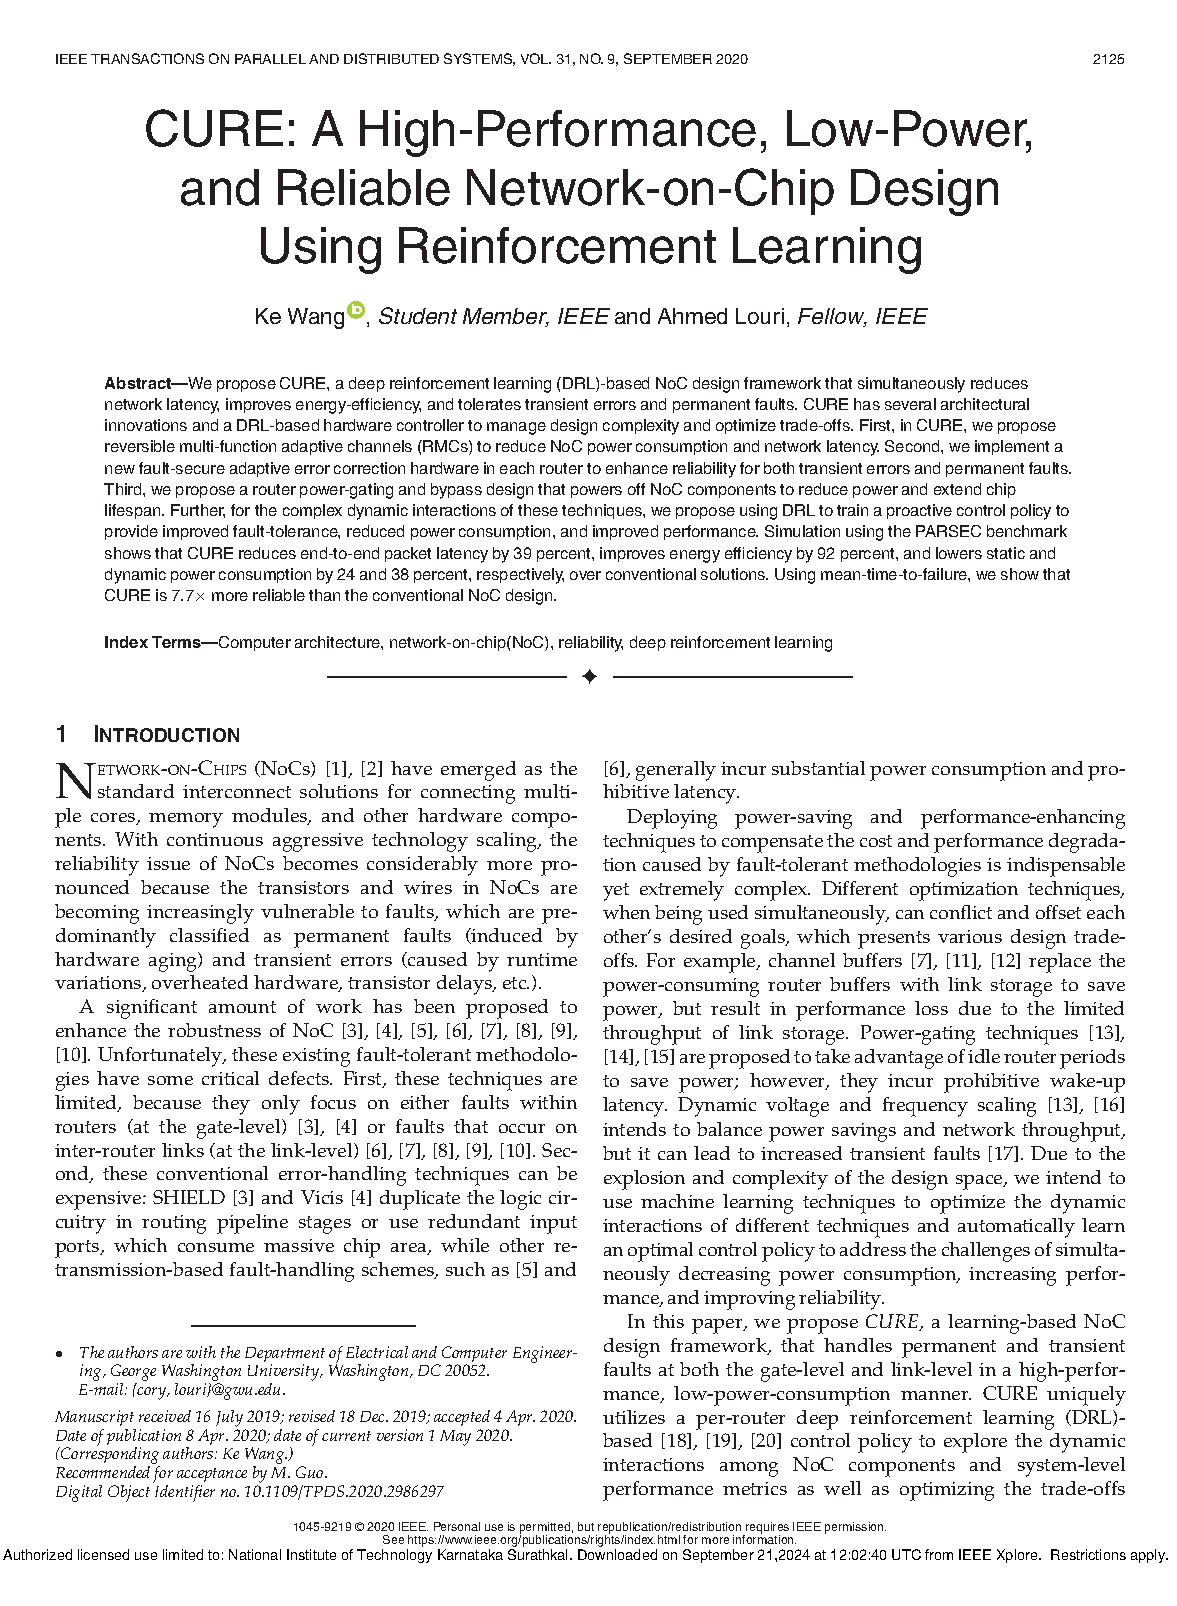
\includegraphics[width=\textwidth]{2.jpg}
		\caption{Chat Flow Step 2:System provides feature explanation .}
		\label{fig:step2}
	\end{minipage}
\end{figure}

\begin{figure}[h!]
	\centering
	\begin{minipage}{0.45\textwidth}
		\centering
		\includegraphics[width=\textwidth]{3.jpg}
		\caption{Chat Flow Step 3: User provides feature values.}
		\label{fig:step3}
	\end{minipage}%
	\hspace{0.05\textwidth} % Add space between the images
	\begin{minipage}{0.45\textwidth}
		\centering
		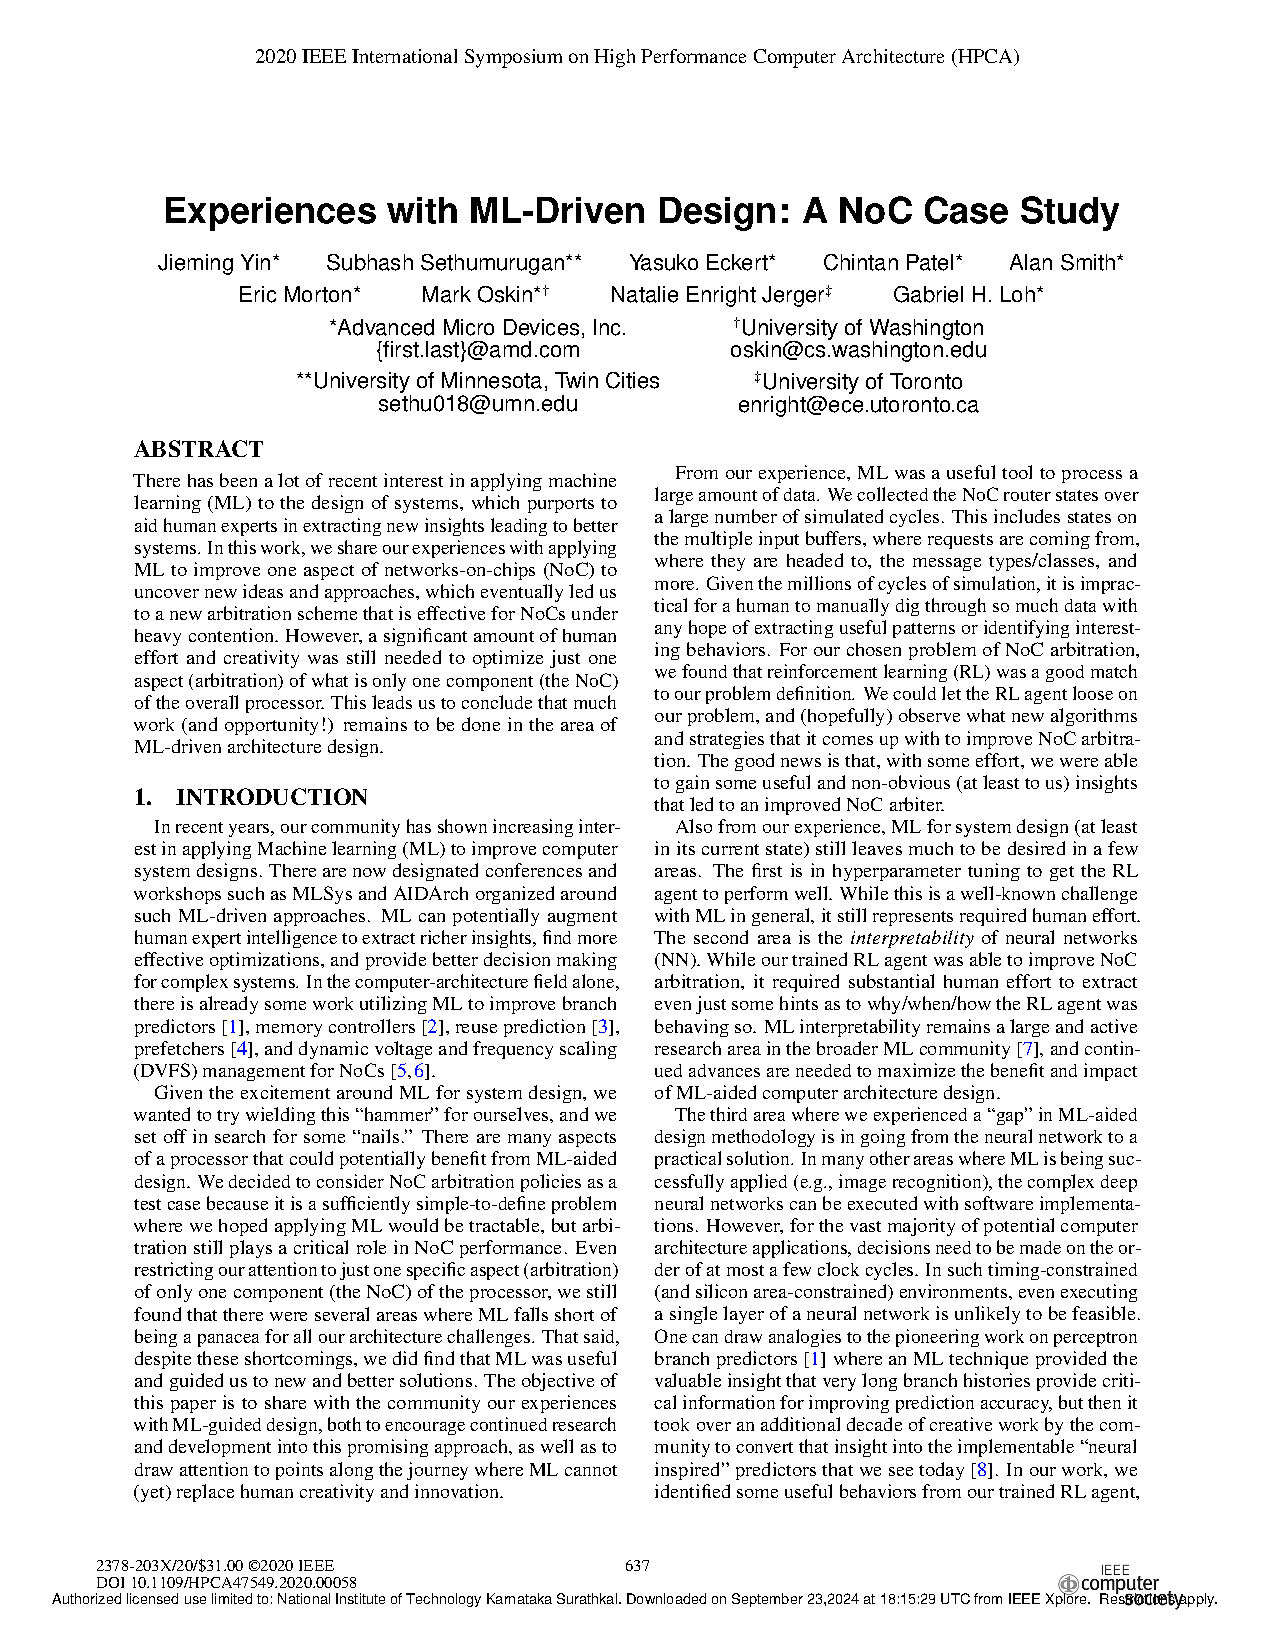
\includegraphics[width=\textwidth]{4.jpg}
		\caption{Chat Flow Step 4: User receives car price prediction and SHAP explanation.}
		\label{fig:step4}
	\end{minipage}
\end{figure}



The above images demonstrate how the chatbot processes requests from the user, predicts the car price, and provides detailed insights into the most influential features that contribute to the price.

In conclusion, the combination of machine learning, SHAP-based explanations, Rasa-powered chatbot, Flask backend, and Telegram frontend provides a comprehensive and effective solution for car price prediction. This system offers users an engaging, transparent, and accessible way to predict car prices, understand the underlying factors influencing those prices, and interact with the model through a conversational interface.

\section{Conclusion}
This project provides an effective and interactive solution for car price prediction using machine learning, integrated with a conversational chatbot. The system leverages a robust machine learning model to predict car prices based on various features such as brand, model, year, and other attributes. By incorporating SHAP (SHapley Additive exPlanations) values, the system enhances transparency by providing users with explanations about the most influential features in the predicted price. The backend is built using Flask, which efficiently handles the interaction between the model and the frontend. The user interacts with the system via a Telegram-based chatbot, which uses Rasa to manage natural language understanding and processing.

Through this approach, users can easily predict car prices and receive valuable insights into the factors influencing those prices. This interactive, user-friendly system enhances the user experience by offering immediate, clear, and detailed responses in real-time. The combination of machine learning, SHAP explanations, Rasa-powered chatbot, Flask backend, and Telegram frontend creates a seamless and engaging solution for car price prediction.

\section{Future Work}
\begin{itemize}
	\item \textbf{Model Enhancement:} The current model can be improved by incorporating more advanced machine learning techniques, such as deep learning models or ensemble methods, to enhance the accuracy of the price predictions. This could further refine the predictions, especially in cases with more complex data relationships.
	
	\item \textbf{Multi-Language Support:} The chatbot can be enhanced to support multiple languages, making the system more accessible to a global audience. This would be particularly useful for non-English speaking regions and increase the chatbot's usability worldwide.
	
	\item \textbf{Integration with Other Platforms:} The system could be expanded to work on other platforms, such as web applications or mobile apps, to reach a wider audience beyond Telegram. A broader platform support would also enhance user accessibility, allowing users to engage with the chatbot through more channels.
	
	\item \textbf{Voice Interaction:} Another potential enhancement is incorporating voice recognition and synthesis. This would allow users to interact with the chatbot via voice commands and receive spoken responses, making the system more interactive and user-friendly, particularly for users on the go.
\end{itemize}




\begin{thebibliography}{9}
	
	\bibitem{rasa}
	Rasa Technologies, ``Rasa Documentation,'' \textit{Rasa}, 2023. [Online]. Available: \texttt{https://rasa.com/docs/}
	\bibitem{flask}
	Armin Ronacher, ``Flask Documentation,'' \textit{Flask}, 2023. [Online]. Available: \texttt{https://flask.palletsprojects.com/}
	
	\bibitem{shap-doc}
	SHAP Documentation, ``SHAP (SHapley Additive exPlanations),'' 2023. [Online]. Available: \texttt{https://shap.readthedocs.io/en/latest/}
	
	\bibitem{randomforest}
	Leo Breiman, ``Random Forests,'' \textit{Machine Learning}, vol. 45, no. 1, 2001, pp. 5-32. [Online]. Available: \texttt{https://link.springer.com/article/10.1023/A:1010933404324}
	
	\bibitem{randomforest-doc}
	Scikit-learn, ``Random Forests,'' 2023. [Online]. Available: \texttt{https://scikit-learn.org/stable/modules/ensemble.html-random-forests}
	
\end{thebibliography}

\end{justify}
\end{document}
